% Options for packages loaded elsewhere
\PassOptionsToPackage{unicode}{hyperref}
\PassOptionsToPackage{hyphens}{url}
%
\documentclass[
  english,
  man]{apa6}
\usepackage{lmodern}
\usepackage{amssymb,amsmath}
\usepackage{ifxetex,ifluatex}
\ifnum 0\ifxetex 1\fi\ifluatex 1\fi=0 % if pdftex
  \usepackage[T1]{fontenc}
  \usepackage[utf8]{inputenc}
  \usepackage{textcomp} % provide euro and other symbols
\else % if luatex or xetex
  \usepackage{unicode-math}
  \defaultfontfeatures{Scale=MatchLowercase}
  \defaultfontfeatures[\rmfamily]{Ligatures=TeX,Scale=1}
\fi
% Use upquote if available, for straight quotes in verbatim environments
\IfFileExists{upquote.sty}{\usepackage{upquote}}{}
\IfFileExists{microtype.sty}{% use microtype if available
  \usepackage[]{microtype}
  \UseMicrotypeSet[protrusion]{basicmath} % disable protrusion for tt fonts
}{}
\makeatletter
\@ifundefined{KOMAClassName}{% if non-KOMA class
  \IfFileExists{parskip.sty}{%
    \usepackage{parskip}
  }{% else
    \setlength{\parindent}{0pt}
    \setlength{\parskip}{6pt plus 2pt minus 1pt}}
}{% if KOMA class
  \KOMAoptions{parskip=half}}
\makeatother
\usepackage{xcolor}
\IfFileExists{xurl.sty}{\usepackage{xurl}}{} % add URL line breaks if available
\IfFileExists{bookmark.sty}{\usepackage{bookmark}}{\usepackage{hyperref}}
\hypersetup{
  pdftitle={An institutional approach to attention allocation and venture resource mobilization and acquisition},
  pdfauthor={Ouafaa Hmaddi1},
  pdfkeywords={attention, resources, institutional capital, accelerators},
  hidelinks,
  pdfcreator={LaTeX via pandoc}}
\urlstyle{same} % disable monospaced font for URLs
\usepackage{graphicx,grffile}
\makeatletter
\def\maxwidth{\ifdim\Gin@nat@width>\linewidth\linewidth\else\Gin@nat@width\fi}
\def\maxheight{\ifdim\Gin@nat@height>\textheight\textheight\else\Gin@nat@height\fi}
\makeatother
% Scale images if necessary, so that they will not overflow the page
% margins by default, and it is still possible to overwrite the defaults
% using explicit options in \includegraphics[width, height, ...]{}
\setkeys{Gin}{width=\maxwidth,height=\maxheight,keepaspectratio}
% Set default figure placement to htbp
\makeatletter
\def\fps@figure{htbp}
\makeatother
\setlength{\emergencystretch}{3em} % prevent overfull lines
\providecommand{\tightlist}{%
  \setlength{\itemsep}{0pt}\setlength{\parskip}{0pt}}
\setcounter{secnumdepth}{-\maxdimen} % remove section numbering
% Make \paragraph and \subparagraph free-standing
\ifx\paragraph\undefined\else
  \let\oldparagraph\paragraph
  \renewcommand{\paragraph}[1]{\oldparagraph{#1}\mbox{}}
\fi
\ifx\subparagraph\undefined\else
  \let\oldsubparagraph\subparagraph
  \renewcommand{\subparagraph}[1]{\oldsubparagraph{#1}\mbox{}}
\fi
% Manuscript styling
\usepackage{upgreek}
\captionsetup{font=singlespacing,justification=justified}

% Table formatting
\usepackage{longtable}
\usepackage{lscape}
% \usepackage[counterclockwise]{rotating}   % Landscape page setup for large tables
\usepackage{multirow}		% Table styling
\usepackage{tabularx}		% Control Column width
\usepackage[flushleft]{threeparttable}	% Allows for three part tables with a specified notes section
\usepackage{threeparttablex}            % Lets threeparttable work with longtable

% Create new environments so endfloat can handle them
% \newenvironment{ltable}
%   {\begin{landscape}\begin{center}\begin{threeparttable}}
%   {\end{threeparttable}\end{center}\end{landscape}}
\newenvironment{lltable}{\begin{landscape}\begin{center}\begin{ThreePartTable}}{\end{ThreePartTable}\end{center}\end{landscape}}

% Enables adjusting longtable caption width to table width
% Solution found at http://golatex.de/longtable-mit-caption-so-breit-wie-die-tabelle-t15767.html
\makeatletter
\newcommand\LastLTentrywidth{1em}
\newlength\longtablewidth
\setlength{\longtablewidth}{1in}
\newcommand{\getlongtablewidth}{\begingroup \ifcsname LT@\roman{LT@tables}\endcsname \global\longtablewidth=0pt \renewcommand{\LT@entry}[2]{\global\advance\longtablewidth by ##2\relax\gdef\LastLTentrywidth{##2}}\@nameuse{LT@\roman{LT@tables}} \fi \endgroup}

% \setlength{\parindent}{0.5in}
% \setlength{\parskip}{0pt plus 0pt minus 0pt}

% \usepackage{etoolbox}
\makeatletter
\patchcmd{\HyOrg@maketitle}
  {\section{\normalfont\normalsize\abstractname}}
  {\section*{\normalfont\normalsize\abstractname}}
  {}{\typeout{Failed to patch abstract.}}
\patchcmd{\HyOrg@maketitle}
  {\section{\protect\normalfont{\@title}}}
  {\section*{\protect\normalfont{\@title}}}
  {}{\typeout{Failed to patch title.}}
\makeatother
\shorttitle{An institutional approach to venture attention allocation}
\keywords{attention, resources, institutional capital, accelerators}
\DeclareDelayedFloatFlavor{ThreePartTable}{table}
\DeclareDelayedFloatFlavor{lltable}{table}
\DeclareDelayedFloatFlavor*{longtable}{table}
\makeatletter
\renewcommand{\efloat@iwrite}[1]{\immediate\expandafter\protected@write\csname efloat@post#1\endcsname{}}
\makeatother
\usepackage{lineno}

\linenumbers
\usepackage{csquotes}
\ifxetex
  % Load polyglossia as late as possible: uses bidi with RTL langages (e.g. Hebrew, Arabic)
  \usepackage{polyglossia}
  \setmainlanguage[]{english}
\else
  \usepackage[shorthands=off,main=english]{babel}
\fi

\title{An institutional approach to attention allocation and venture resource mobilization and acquisition}
\author{Ouafaa Hmaddi\textsuperscript{1}}
\date{}


\authornote{

Lundquist College of Business

Department of Management

The authors made the following contributions. Ouafaa Hmaddi: Conceptualization, Writing - Original Draft Preparation, Writing - Review \& Editing.

Correspondence concerning this article should be addressed to Ouafaa Hmaddi, 292A Anstett. E-mail: \href{mailto:ohmaddi@uoregon.edu}{\nolinkurl{ohmaddi@uoregon.edu}}

}

\affiliation{\vspace{0.5cm}\textsuperscript{1} University of Oregon}

\abstract{
One or two sentences providing a \textbf{basic introduction} to the field, comprehensible to a scientist in any discipline.
}



\begin{document}
\maketitle

\hypertarget{introduction}{%
\section{Introduction}\label{introduction}}

Early stage entrepreneurs are faced with a range of resource choices to seek, and must decide what should garner their attention. The literature on entrepreneurial resources argues the resources entrepreneurs possess shape their resource acquisition and once they raise one resource others follow. Thus, one might theorize that founders should focus their attention on the resource they can leverage based on their existing resource endowment. However, resource acquisition depends on both entrepreneurs' resource endowment and the institutional-level capital. Both are indispensable antecedents that affect the mobilization and acquisition of additional capital.

The value of a resource varies with its institutional context (Holburn \& Zelner, 2010). On the one hand, strong institutions can increase the value of a resource by streamlining access to complementary external resources (Khanna \& Rivkin, 2001; North \& others, 1990). For example, in countries with strong financing infrastructure, acquiring financing can streamline accessing other resources and thus it would make sense to focus on raising capital at venture's earliest stages. On the other hand, resources such as legitimation or social capital can substitute for the weak institutions and capital infrastructure, thereby increasing in value when institutions are weak (Khanna \& Palepu, 1997; Kock \& Guillén, 2001). Therefore, the broader environment can enhance or inhibit the optimal use of the endowed resource capital. I posit that an examination of both the venture and its broader institutional environment would give us more insights about where founders attention should be allocated. Specifically, I hypothesize that the institutional-level capital positively moderates the relationship between a founder's attention and its subsequent resource mobilization and acquisition. For example, attention to human capital is more positively related to a higher number of employees in contexts in which it has higher intuitional-level human capital. This similarly applies to social capital, and financial capital as the types of resources sought by entrepreneurs. Thus, in this paper I seek to examine the following research question: How does the alignment of the institutional context and the allocation of entrepreneurial attention toward specific resources influence the venture's resource mobilization and acquisition?

\hypertarget{hypotheses-development}{%
\section{Hypotheses Development}\label{hypotheses-development}}

At the heart of the intersection between resource acquisition and the institutional context is entrepreneurial attention, that is, founders' attention allocation to resources. Bounded by their limited attentional capacities, entrepreneurs cannot attend to all the resources; rather, they focus on some resources but must ignore others. Where they focus their attention determines the propensity of mobilizing and acquiring resources. A venture could miss the chance to exploit an opportunity of resources acquisition if that opportunity never appears on the entrepreneur's radar screens because they are too focused on an alternative resource. For example, a voluntary work with potential partners who are well connected to other investors might be missed because the founder is too focused on raising capital by honing their business plan over and over and even paying accounting boutique firms to develop that business plan for them.

Thus, selective attention plays a crucial role in both individual and organizational behavior because it bounds individual rationality and determines the menu of available actions (Simon, 1947). The debate over which resource should garner the entrepreneur's attention concludes that the founding team resource endowment is the key factor that influences resource acquisition. For instance, scholars argue that founding teams with a more ties to potential investors are more likely to gain funding (Shane \& Stuart, 2002). Furthermore, if we focus on the findings of the stream of research examining the performance implications of acquiring financial capital (e.g.; (Hochberg, Ljungqvist, \& Lu, 2007)) we would expect that early-stage financing should be most likely to garner founders' attention. However, the role of the institutional context has been ignored and neglected in this debate. I argue that selective attention allocation depends on both entrepreneur's resource endowment and institutional capital.

Therefore, I state the following hypotheses about the relationship between the congruence level of the entrepreneurs' attention to resources and the institutional level capital, and the venture's resource mobilization, acquisition, and performance.

\textbf{Hypothesis 1} \emph{The higher the level of congruency of venture's attention to a resource and its institutional level capital, the higher the odds of mobilization that resource}

\textbf{Hypothesis 2} \emph{The higher the level of congruency of venture's attention to a resource and its institutional level capital, the higher the level of the accumulated resource}

\textbf{Hypothesis 3} \emph{The higher the level of congruency of venture's attention to a resource and its institutional level capital, the higher the venture performance}

\hypertarget{analysis}{%
\section{Analysis}\label{analysis}}

\hypertarget{measures}{%
\subsection{Measures}\label{measures}}

\hypertarget{data}{%
\subsection{Data}\label{data}}

\hypertarget{methods}{%
\subsection{Methods}\label{methods}}

We report how we determined our sample size, all data exclusions (if any), all manipulations, and all measures in the study.

\hypertarget{data-analysis}{%
\subsection{Data analysis}\label{data-analysis}}

I used R (Version 4.0.2; R Core Team, 2020b) and the R-packages \emph{caret} (Version 6.0.86; Kuhn, 2020), \emph{dplyr} (Version 1.0.0; Wickham et al., 2020), \emph{EFAutilities} (Version 2.0.0; Zhang, Jiang, Hattori, \& Trichtinger, 2019), \emph{forcats} (Version 0.5.0; Wickham, 2020), \emph{foreign} (Version 0.8.80; R Core Team, 2020a), \emph{ggplot2} (Version 3.3.2; Wickham, 2016), \emph{haven} (Version 2.3.1; Wickham \& Miller, 2020), \emph{janitor} (Version 2.0.1; Firke, 2020), \emph{knitr} (Version 1.29; Xie, 2015), \emph{lattice} (Version 0.20.41; Sarkar, 2008), \emph{lme4} (Version 1.1.23; Bates, Mächler, Bolker, \& Walker, 2015), \emph{lmerTest} (Version 3.1.2; Kuznetsova, Brockhoff, \& Christensen, 2017), \emph{lubridate} (Version 1.7.9; Grolemund \& Wickham, 2011), \emph{Matrix} (Version 1.2.18; Bates \& Maechler, 2019), \emph{papaja} (Version 0.1.0.9997; Aust \& Barth, 2020), \emph{plm} (Version 2.2.3; Croissant \& Millo, 2008; Millo, 2017), \emph{plot3D} (Version 1.3; Soetaert, 2019), \emph{preprocessCore} (Version 1.50.0; Bolstad, 2020), \emph{psych} (Version 1.9.12.31; Revelle, 2019), \emph{purrr} (Version 0.3.4; Henry \& Wickham, 2020), \emph{readr} (Version 1.3.1; Wickham, Hester, \& Francois, 2018), \emph{readxl} (Version 1.3.1; Wickham \& Bryan, 2019), \emph{reshape2} (Version 1.4.4; Wickham, 2007), \emph{rio} (Version 0.5.16; Chan, Chan, Leeper, \& Becker, 2018), \emph{sjPlot} (Version 2.8.4; Lüdecke, 2020), \emph{stringr} (Version 1.4.0; Wickham, 2019), \emph{tibble} (Version 3.0.3; Müller \& Wickham, 2020), \emph{tidyr} (Version 1.1.0; Wickham \& Henry, 2020), \emph{tidyverse} (Version 1.3.0; Wickham, Averick, et al., 2019), and \emph{XLConnect} (Version 1.0.1; Mirai Solutions GmbH, 2020) for all our analyses.

\#CGI data

\#Plotting all countries along the 3 dimensions

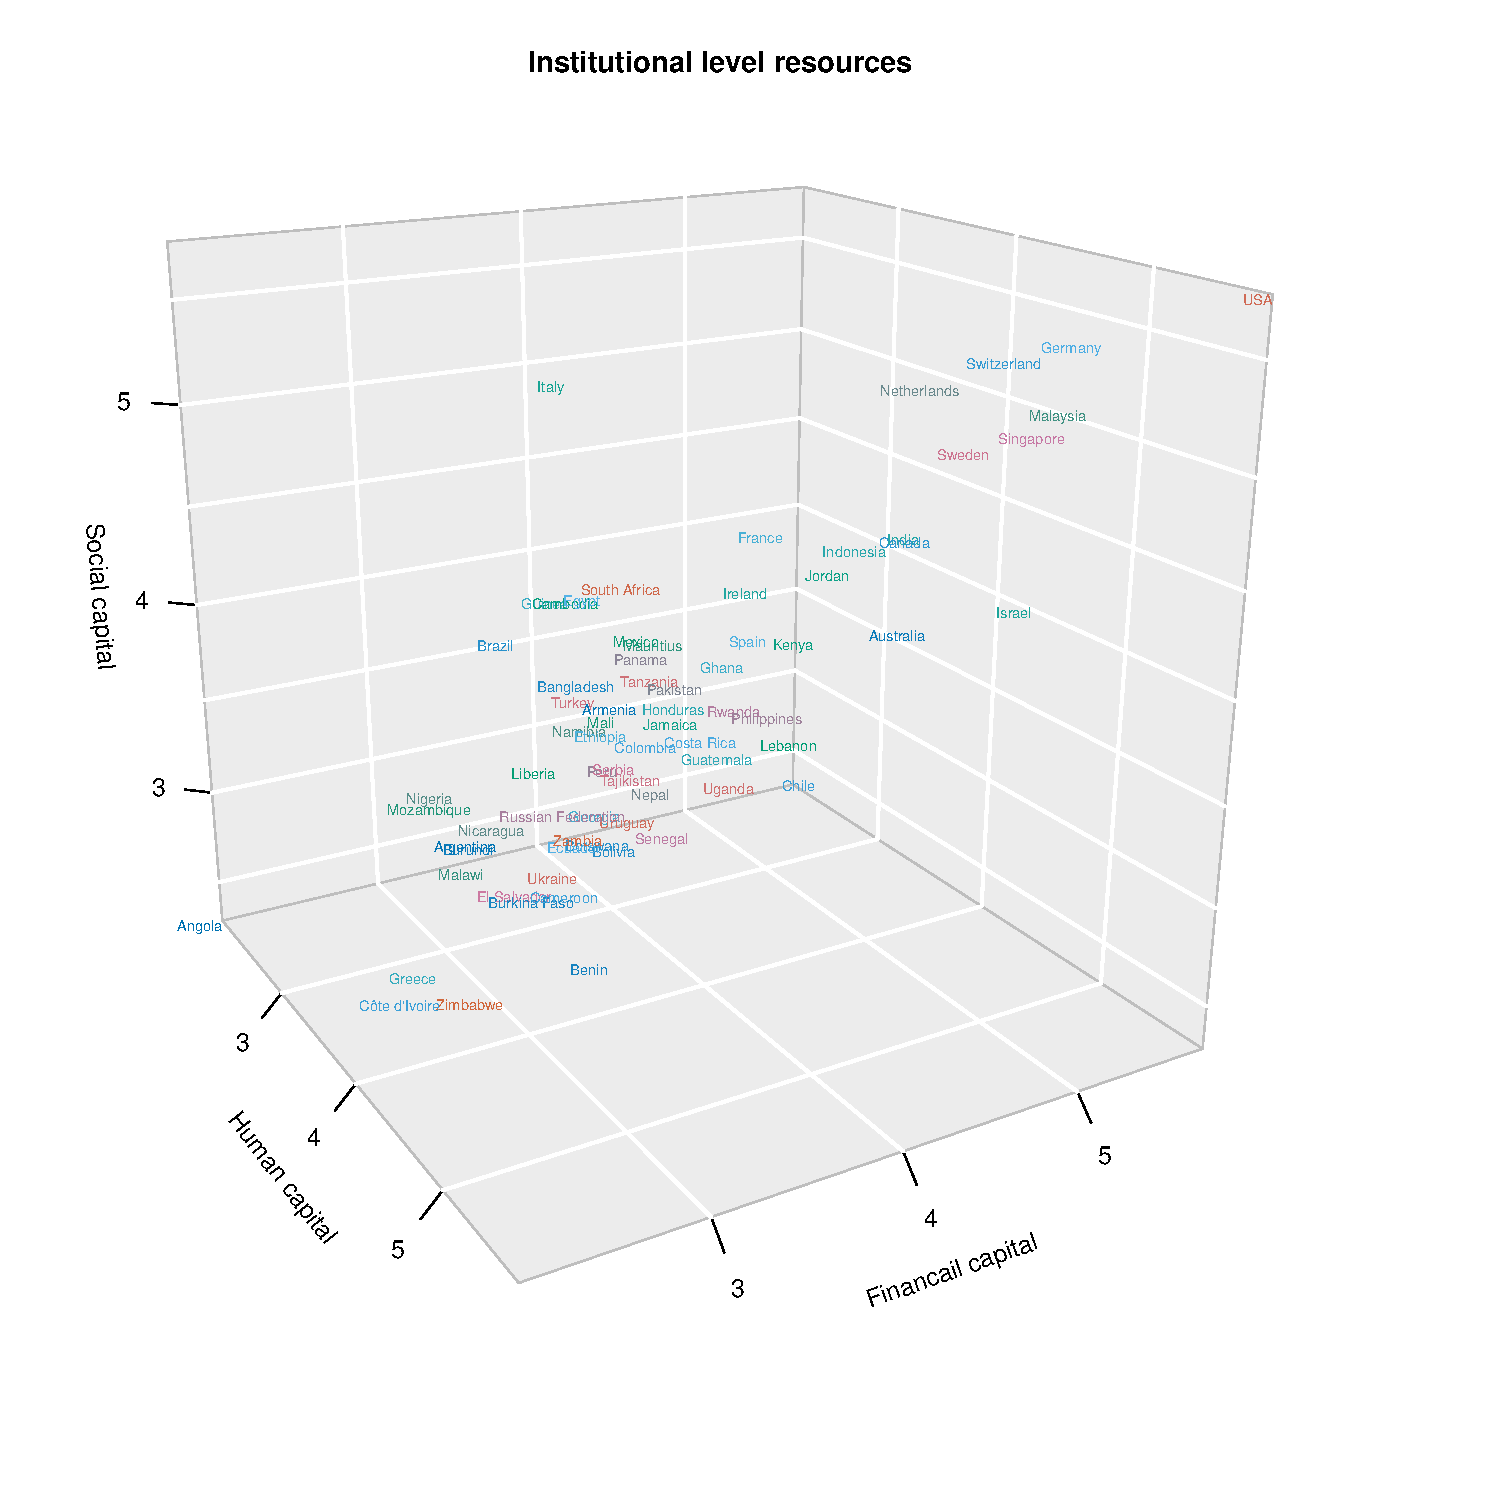
\includegraphics{Manuscript_files/figure-latex/unnamed-chunk-4-1.pdf} 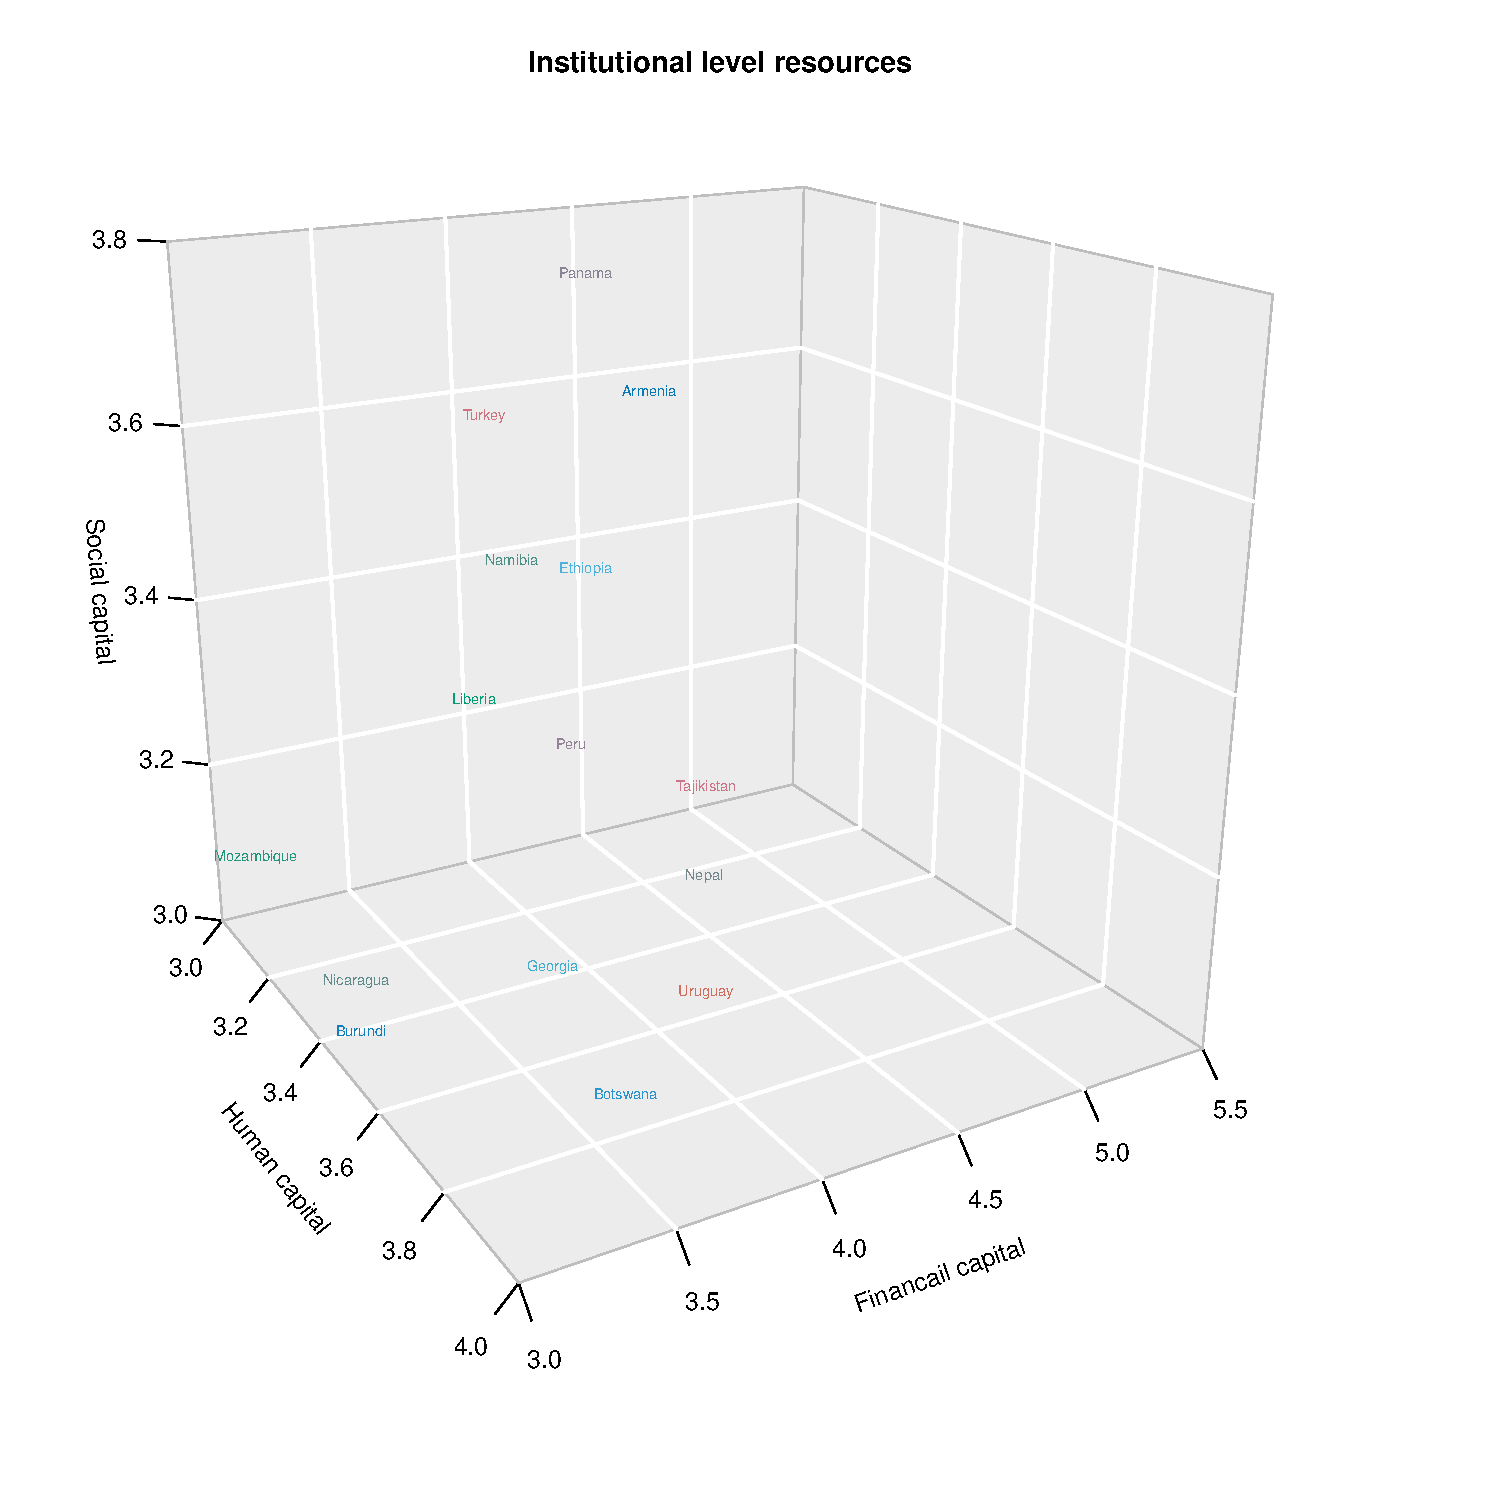
\includegraphics{Manuscript_files/figure-latex/unnamed-chunk-4-2.pdf}

\#Attention to capital - venture data

\#\#Control variables

\#\#Constrcuting human capital index (control variable)
\#\#\#Graduate percentage, Prior C-level Executive Percentage, Average Team Tenure , Team Prior Founding

\#\#Gender decomposition variable

\#Reverse code attention variable

\#Distribution of attention

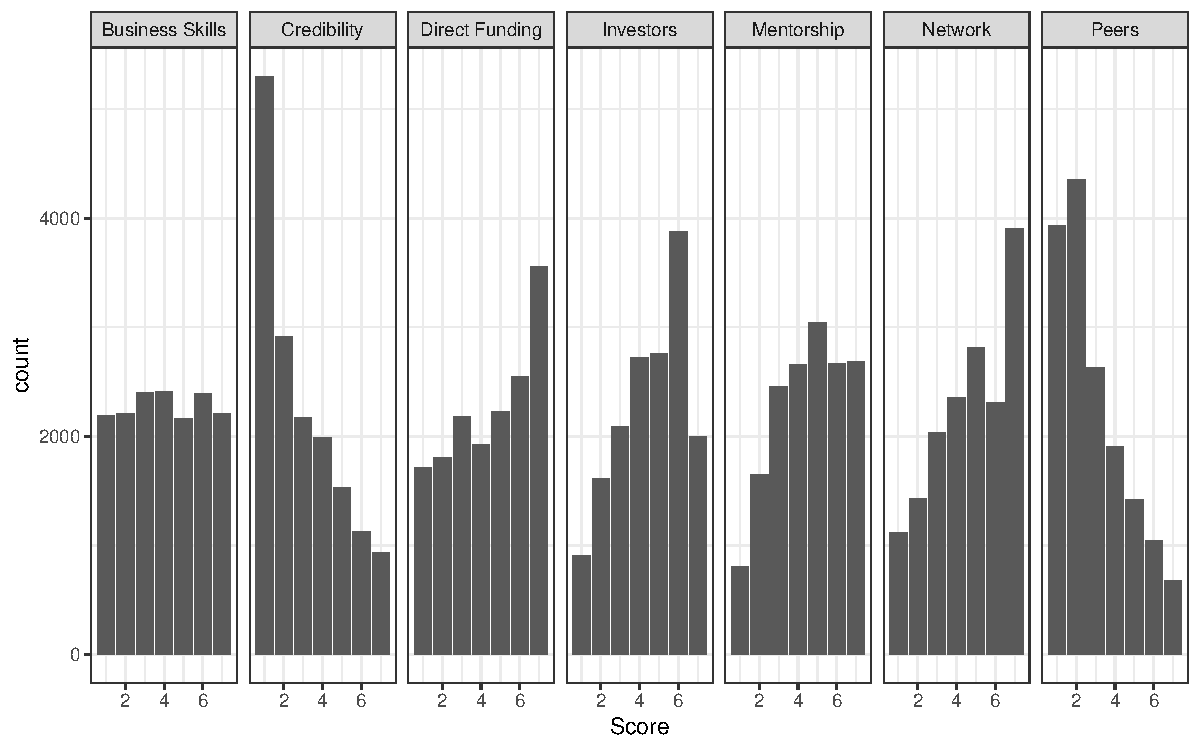
\includegraphics{Manuscript_files/figure-latex/unnamed-chunk-6-1.pdf} 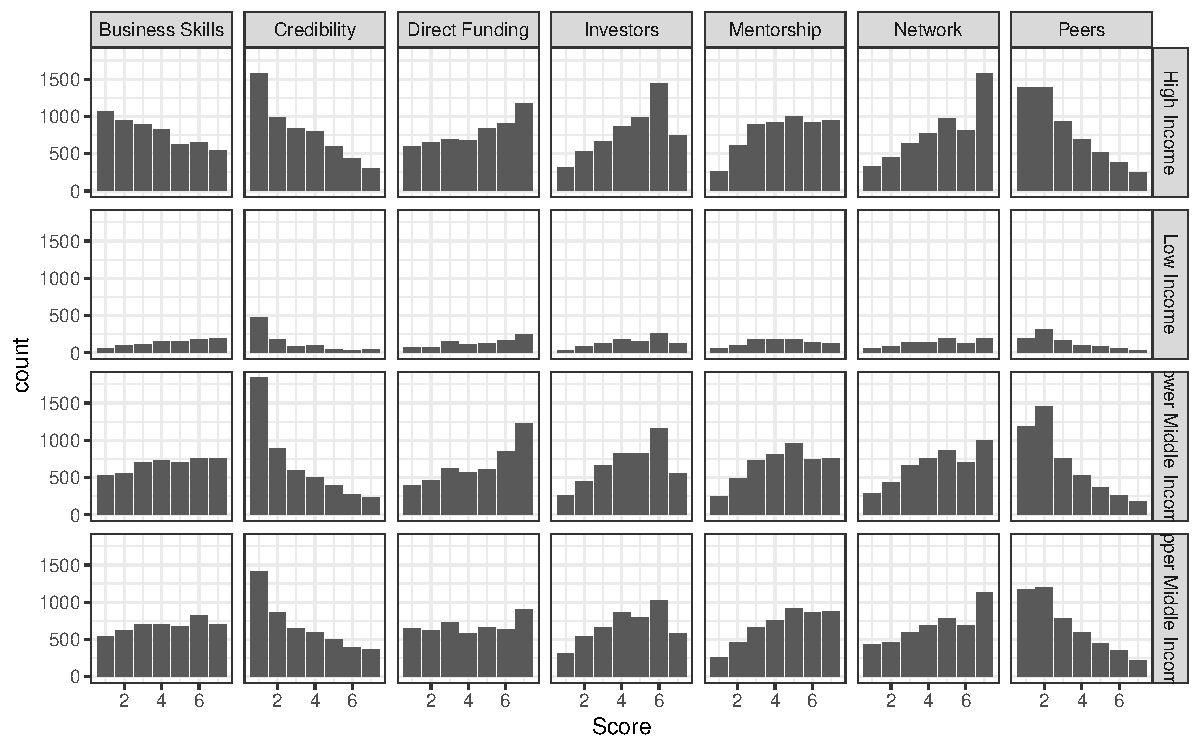
\includegraphics{Manuscript_files/figure-latex/unnamed-chunk-6-2.pdf}

\#\#Outcomes

\#Revenues

\#Human capital acquisition

\#Social capital acquisition

\#Fiancial Capital acquisiton total

\#Predictor and outcome plots
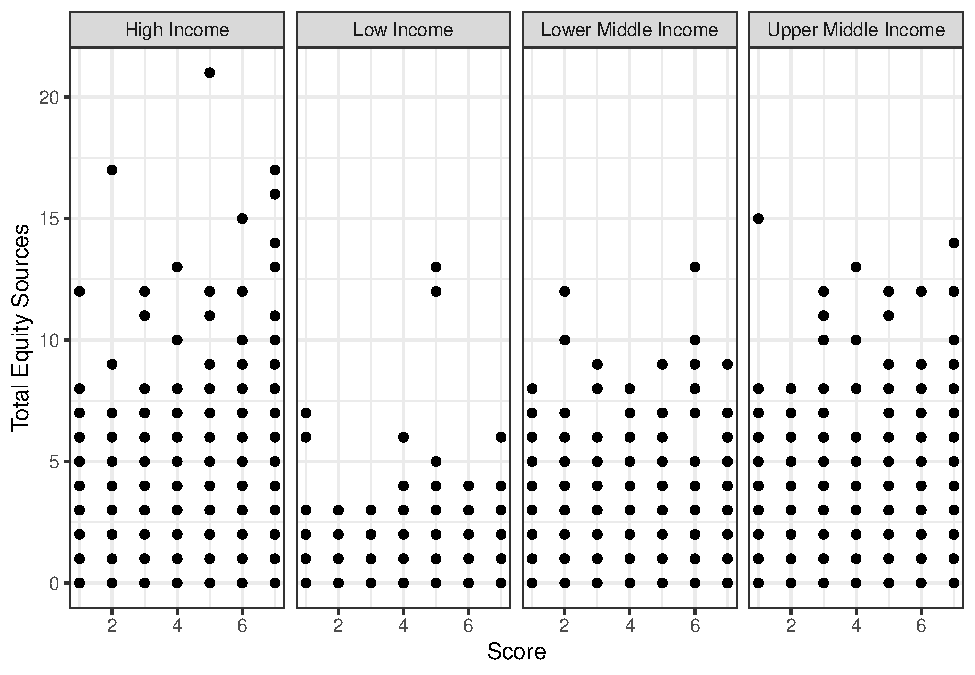
\includegraphics{Manuscript_files/figure-latex/unnamed-chunk-11-1.pdf} 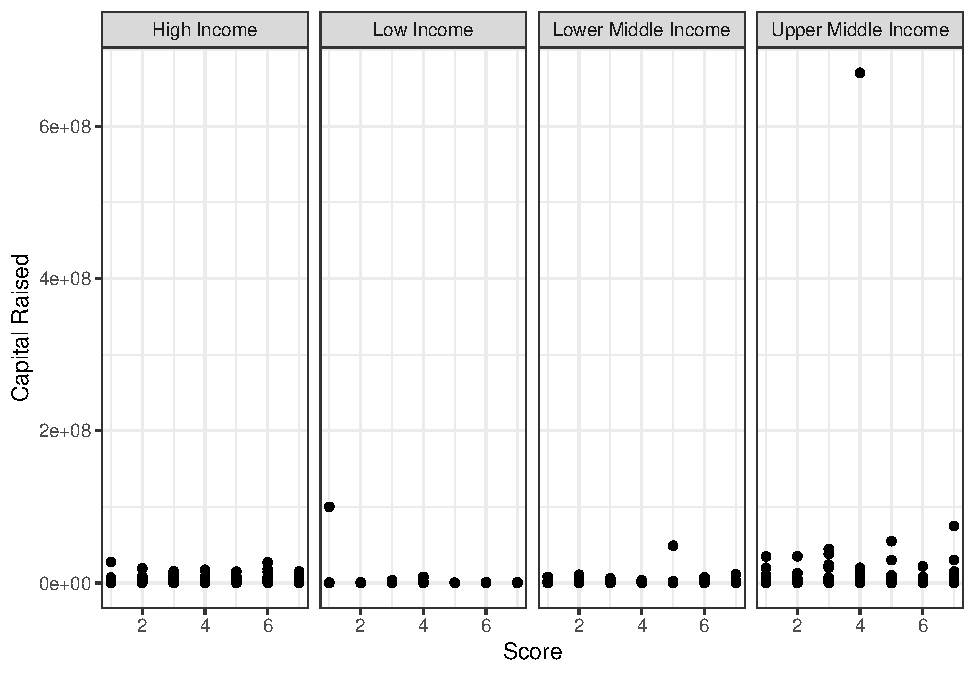
\includegraphics{Manuscript_files/figure-latex/unnamed-chunk-11-2.pdf}

\#Join all 3 datasets

\hypertarget{results}{%
\section{Results}\label{results}}

\#Mixed model analysis - Human capital

\begin{tabular}{l|l|l|l}
\hline
  & $b$ & SE & $z$\\
\hline
Intercept & -1.46 & 0.08 & -19.18\\
\hline
Attention to Human capital(AHC) & 0.11 & 0.07 & 1.54\\
\hline
\end{tabular}

\begin{tabular}{l|l|l|l}
\hline
  & $b$ & SE & $z$\\
\hline
Intercept & -0.85 & 0.53 & -1.61\\
\hline
AHC & 0.92 & 0.45 & 2.05\\
\hline
Ease of finding skilled employees & -0.14 & 0.12 & -1.14\\
\hline
AHCxEase of finding skilled employees & -0.17 & 0.10 & -1.79\\
\hline
\end{tabular}

\begin{tabular}{l|l|l|l}
\hline
  & $b$ & SE & $t$\\
\hline
Intercept & 762.25 & 502.25 & 1.52\\
\hline
Attention to Human capital & 2,955.97 & 2,238.11 & 1.32\\
\hline
\end{tabular}

\begin{tabular}{l|l|l|l}
\hline
  & $b$ & SE & $t$\\
\hline
Intercept & -1,955.91 & 3,599.05 & -0.54\\
\hline
AHC & -10,174.65 & 16,704.03 & -0.61\\
\hline
Ease of finding skilled employees & 641.03 & 813.08 & 0.79\\
\hline
AHCxEase of finding skilled employees & 3,118.93 & 3,842.90 & 0.81\\
\hline
\end{tabular}

\#Mixed model analysis - Financial capital

\begin{verbatim}
## Generalized linear mixed model fit by maximum likelihood (Laplace
##   Approximation) [glmerMod]
##  Family: binomial  ( logit )
## Formula: 
## participated ~ accel_ben_rank_direct_funding + (accel_ben_rank_direct_funding |  
##     country)
##    Data: gali_joined
## 
##      AIC      BIC   logLik deviance df.resid 
##  14773.7  14812.1  -7381.8  14763.7    15976 
## 
## Scaled residuals: 
##     Min      1Q  Median      3Q     Max 
## -1.0388 -0.4890 -0.4207 -0.3515  3.0479 
## 
## Random effects:
##  Groups  Name                          Variance Std.Dev. Corr 
##  country (Intercept)                   0.300861 0.54851       
##          accel_ben_rank_direct_funding 0.007982 0.08934  -1.00
## Number of obs: 15981, groups:  country, 82
## 
## Fixed effects:
##                               Estimate Std. Error z value Pr(>|z|)    
## (Intercept)                   -1.45326    0.07722 -18.821  < 2e-16 ***
## accel_ben_rank_direct_funding -0.19333    0.06321  -3.059  0.00222 ** 
## ---
## Signif. codes:  0 '***' 0.001 '**' 0.01 '*' 0.05 '.' 0.1 ' ' 1
## 
## Correlation of Fixed Effects:
##             (Intr)
## accl_bn_r__ -0.171
## convergence code: 0
## boundary (singular) fit: see ?isSingular
\end{verbatim}

\begin{verbatim}
## Generalized linear mixed model fit by maximum likelihood (Laplace
##   Approximation) [glmerMod]
##  Family: binomial  ( logit )
## Formula: 
## participated ~ accel_ben_rank_direct_funding * EOSQ425 + (accel_ben_rank_direct_funding |  
##     country)
##    Data: gali_joined
## 
##      AIC      BIC   logLik deviance df.resid 
##  14562.1  14615.8  -7274.1  14548.1    15720 
## 
## Scaled residuals: 
##     Min      1Q  Median      3Q     Max 
## -1.0463 -0.4908 -0.4210 -0.3513  3.0165 
## 
## Random effects:
##  Groups  Name                          Variance Std.Dev. Corr 
##  country (Intercept)                   0.287438 0.53613       
##          accel_ben_rank_direct_funding 0.009936 0.09968  -1.00
## Number of obs: 15727, groups:  country, 73
## 
## Fixed effects:
##                                        Estimate Std. Error z value Pr(>|z|)   
## (Intercept)                           -1.349694   0.434021  -3.110  0.00187 **
## accel_ben_rank_direct_funding         -0.210801   0.285396  -0.739  0.46013   
## EOSQ425                               -0.021755   0.112408  -0.194  0.84654   
## accel_ben_rank_direct_funding:EOSQ425  0.003382   0.065751   0.051  0.95898   
## ---
## Signif. codes:  0 '***' 0.001 '**' 0.01 '*' 0.05 '.' 0.1 ' ' 1
## 
## Correlation of Fixed Effects:
##             (Intr) ac____ EOSQ42
## accl_bn_r__ -0.246              
## EOSQ425     -0.983  0.246       
## a____:EOSQ4  0.280 -0.974 -0.289
## convergence code: 0
## boundary (singular) fit: see ?isSingular
\end{verbatim}

\begin{verbatim}
## Generalized linear mixed model fit by maximum likelihood (Laplace
##   Approximation) [glmerMod]
##  Family: binomial  ( logit )
## Formula: 
## participated ~ accel_ben_rank_direct_funding * EOSQ089 + (accel_ben_rank_direct_funding |  
##     country)
##    Data: gali_joined
## 
##      AIC      BIC   logLik deviance df.resid 
##  14561.6  14615.2  -7273.8  14547.6    15720 
## 
## Scaled residuals: 
##     Min      1Q  Median      3Q     Max 
## -1.0482 -0.4904 -0.4209 -0.3510  3.0323 
## 
## Random effects:
##  Groups  Name                          Variance Std.Dev. Corr 
##  country (Intercept)                   0.284084 0.53299       
##          accel_ben_rank_direct_funding 0.009676 0.09837  -1.00
## Number of obs: 15727, groups:  country, 73
## 
## Fixed effects:
##                                       Estimate Std. Error z value Pr(>|z|)    
## (Intercept)                           -1.21998    0.28033  -4.352 1.35e-05 ***
## accel_ben_rank_direct_funding         -0.24283    0.19650  -1.236    0.217    
## EOSQ089                               -0.07084    0.09006  -0.787    0.432    
## accel_ben_rank_direct_funding:EOSQ089  0.01463    0.05184   0.282    0.778    
## ---
## Signif. codes:  0 '***' 0.001 '**' 0.01 '*' 0.05 '.' 0.1 ' ' 1
## 
## Correlation of Fixed Effects:
##             (Intr) ac____ EOSQ08
## accl_bn_r__ -0.232              
## EOSQ089     -0.960  0.230       
## a____:EOSQ0  0.281 -0.944 -0.300
## convergence code: 0
## boundary (singular) fit: see ?isSingular
\end{verbatim}

\begin{verbatim}
## Generalized linear mixed model fit by maximum likelihood (Laplace
##   Approximation) [glmerMod]
##  Family: binomial  ( logit )
## Formula: participated ~ accel_ben_rank_direct_funding * DOMCREDITGDP +  
##     (accel_ben_rank_direct_funding | country)
##    Data: gali_joined
## 
##      AIC      BIC   logLik deviance df.resid 
##  14561.8  14615.5  -7273.9  14547.8    15720 
## 
## Scaled residuals: 
##     Min      1Q  Median      3Q     Max 
## -1.0466 -0.4909 -0.4213 -0.3514  3.0629 
## 
## Random effects:
##  Groups  Name                          Variance Std.Dev. Corr 
##  country (Intercept)                   0.289392 0.53795       
##          accel_ben_rank_direct_funding 0.009926 0.09963  -1.00
## Number of obs: 15727, groups:  country, 73
## 
## Fixed effects:
##                                              Estimate Std. Error z value
## (Intercept)                                -1.3735020  0.1256629 -10.930
## accel_ben_rank_direct_funding              -0.2051438  0.1031016  -1.990
## DOMCREDITGDP                               -0.0010317  0.0017273  -0.597
## accel_ben_rank_direct_funding:DOMCREDITGDP  0.0001439  0.0009667   0.149
##                                            Pr(>|z|)    
## (Intercept)                                  <2e-16 ***
## accel_ben_rank_direct_funding                0.0466 *  
## DOMCREDITGDP                                 0.5503    
## accel_ben_rank_direct_funding:DOMCREDITGDP   0.8817    
## ---
## Signif. codes:  0 '***' 0.001 '**' 0.01 '*' 0.05 '.' 0.1 ' ' 1
## 
## Correlation of Fixed Effects:
##             (Intr) ac____ DOMCRE
## accl_bn_r__ -0.193              
## DOMCREDITGD -0.778  0.159       
## a____:DOMCR  0.233 -0.779 -0.313
## convergence code: 0
## boundary (singular) fit: see ?isSingular
\end{verbatim}

\begin{verbatim}
## Linear mixed model fit by maximum likelihood  ['lmerMod']
## Formula: capital_raised_tot ~ +(accel_ben_rank_direct_funding | country)
##    Data: gali_joined
## 
##       AIC       BIC    logLik  deviance  df.resid 
##  541645.1  541683.5 -270817.5  541635.1     15976 
## 
## Scaled residuals: 
##     Min      1Q  Median      3Q     Max 
##  -0.316  -0.040  -0.029  -0.018 120.803 
## 
## Random effects:
##  Groups   Name                          Variance  Std.Dev. Corr
##  country  (Intercept)                   1.187e+11  344600      
##           accel_ben_rank_direct_funding 2.332e+09   48286  1.00
##  Residual                               3.062e+13 5533830      
## Number of obs: 15981, groups:  country, 82
## 
## Fixed effects:
##             Estimate Std. Error t value
## (Intercept)   226024      79869    2.83
## convergence code: 0
## boundary (singular) fit: see ?isSingular
\end{verbatim}

\begin{verbatim}
## Linear mixed model fit by maximum likelihood  ['lmerMod']
## Formula: capital_raised_tot ~ accel_ben_rank_direct_funding * EOSQ425 +  
##     (accel_ben_rank_direct_funding | country)
##    Data: gali_joined
## 
##       AIC       BIC    logLik  deviance  df.resid 
##  533280.8  533342.1 -266632.4  533264.8     15719 
## 
## Scaled residuals: 
##     Min      1Q  Median      3Q     Max 
##  -0.311  -0.041  -0.028  -0.016 119.888 
## 
## Random effects:
##  Groups   Name                          Variance  Std.Dev. Corr
##  country  (Intercept)                   1.247e+11  353102      
##           accel_ben_rank_direct_funding 2.606e+09   51053  1.00
##  Residual                               3.109e+13 5575911      
## Number of obs: 15727, groups:  country, 73
## 
## Fixed effects:
##                                       Estimate Std. Error t value
## (Intercept)                              -4885     444377  -0.011
## accel_ben_rank_direct_funding          -191024     590675  -0.323
## EOSQ425                                  59478     112868   0.527
## accel_ben_rank_direct_funding:EOSQ425    31388     134942   0.233
## 
## Correlation of Fixed Effects:
##             (Intr) ac____ EOSQ42
## accl_bn_r__  0.106              
## EOSQ425     -0.982 -0.103       
## a____:EOSQ4 -0.111 -0.975  0.111
## convergence code: 0
## boundary (singular) fit: see ?isSingular
\end{verbatim}

\begin{verbatim}
## Linear mixed model fit by maximum likelihood  ['lmerMod']
## Formula: capital_raised_tot ~ accel_ben_rank_direct_funding * EOSQ089 +  
##     (accel_ben_rank_direct_funding | country)
##    Data: gali_joined
## 
##       AIC       BIC    logLik  deviance  df.resid 
##  533280.7  533342.0 -266632.3  533264.7     15719 
## 
## Scaled residuals: 
##     Min      1Q  Median      3Q     Max 
##  -0.310  -0.041  -0.028  -0.015 119.888 
## 
## Random effects:
##  Groups   Name                          Variance  Std.Dev. Corr
##  country  (Intercept)                   1.245e+11  352894      
##           accel_ben_rank_direct_funding 2.412e+09   49109  1.00
##  Residual                               3.109e+13 5575889      
## Number of obs: 15727, groups:  country, 73
## 
## Fixed effects:
##                                       Estimate Std. Error t value
## (Intercept)                              66014     285162   0.231
## accel_ben_rank_direct_funding          -205433     401458  -0.512
## EOSQ089                                  51858      88843   0.584
## accel_ben_rank_direct_funding:EOSQ089    41162     104375   0.394
## 
## Correlation of Fixed Effects:
##             (Intr) ac____ EOSQ08
## accl_bn_r__  0.083              
## EOSQ089     -0.957 -0.080       
## a____:EOSQ0 -0.094 -0.944  0.098
## convergence code: 0
## boundary (singular) fit: see ?isSingular
\end{verbatim}

\begin{verbatim}
## Linear mixed model fit by maximum likelihood  ['lmerMod']
## Formula: capital_raised_tot ~ accel_ben_rank_direct_funding * DOMCREDITGDP +  
##     (accel_ben_rank_direct_funding | country)
##    Data: gali_joined
## 
##       AIC       BIC    logLik  deviance  df.resid 
##  533280.9  533342.2 -266632.4  533264.9     15719 
## 
## Scaled residuals: 
##     Min      1Q  Median      3Q     Max 
##  -0.310  -0.041  -0.028  -0.016 119.887 
## 
## Random effects:
##  Groups   Name                          Variance  Std.Dev. Corr
##  country  (Intercept)                   1.245e+11  352820      
##           accel_ben_rank_direct_funding 2.381e+09   48795  1.00
##  Residual                               3.109e+13 5575926      
## Number of obs: 15727, groups:  country, 73
## 
## Fixed effects:
##                                             Estimate Std. Error t value
## (Intercept)                                 190993.0   128015.3   1.492
## accel_ben_rank_direct_funding              -121351.9   210078.0  -0.578
## DOMCREDITGDP                                   572.9     1620.3   0.354
## accel_ben_rank_direct_funding:DOMCREDITGDP     768.4     1952.7   0.393
## 
## Correlation of Fixed Effects:
##             (Intr) ac____ DOMCRE
## accl_bn_r__  0.058              
## DOMCREDITGD -0.761 -0.043       
## a____:DOMCR -0.062 -0.776  0.085
## convergence code: 0
## boundary (singular) fit: see ?isSingular
\end{verbatim}

\#Mixed model analysis - Social capital

\begin{verbatim}
##                          Estimate  Std. Error   t value
## (Intercept)            0.20316446 0.012552069 16.185735
## accel_ben_rank_network 0.01831386 0.009581619  1.911353
\end{verbatim}

\begin{verbatim}
##                                     Estimate Std. Error      t value
## (Intercept)                     3.133837e-01 0.06847055  4.576912615
## accel_ben_rank_network          1.746818e-02 0.05079577  0.343890367
## EOSQ109                        -2.763492e-02 0.01732516 -1.595074599
## accel_ben_rank_network:EOSQ109 -4.430267e-05 0.01131854 -0.003914168
\end{verbatim}

\begin{verbatim}
##                          Estimate Std. Error   t value
## (Intercept)            0.57925930 0.04337800 13.353759
## accel_ben_rank_network 0.06485941 0.04797524  1.351935
\end{verbatim}

\begin{verbatim}
##                                  Estimate Std. Error   t value
## (Intercept)                    -0.2751093 0.21194630 -1.298014
## accel_ben_rank_network         -0.6038282 0.24619417 -2.452650
## EOSQ109                         0.2185398 0.05339006  4.093266
## accel_ben_rank_network:EOSQ109  0.1708510 0.05804559  2.943393
\end{verbatim}

\hypertarget{data-and-methods}{%
\section{Data and Methods}\label{data-and-methods}}

Our dataset, the Global Accelerator Learning Initiative (GALI), covers entrepreneurs who applied to scores of accelerators that began accepting applications between 2013 and 2020. Our data include information -- collected during program applications -- about ventures, founding teams, and pre-program performance. They also identify which applicants went on to participate in each program. Finally, these data include follow-up information collected from selected and rejected applicants in the years following each application window. The anonymized dataset containing both application and follow-up data can be accessed at \href{www.galidata.org/data-request}{GALI Data}.

When entrepreneurs apply to a GALI-participating accelerator, they are asked to complete a standardized survey which asks basic questions about their venture's business model, financial performance, and founding team. Then, after one year, they are asked to complete a follow-up survey, whether or not they were accepted into the program to which they applied.

All financial statistics are in United States Dollars (USD).

Table 1: Ventures in sample, by country of operation and survey responses

\hypertarget{discussion}{%
\section{Discussion}\label{discussion}}

\newpage

\hypertarget{references}{%
\section{References}\label{references}}

\begingroup
\setlength{\parindent}{-0.5in}
\setlength{\leftskip}{0.5in}

\hypertarget{refs}{}
\leavevmode\hypertarget{ref-R-papaja}{}%
Aust, F., \& Barth, M. (2020). \emph{papaja: Create APA manuscripts with R Markdown}. Retrieved from \url{https://github.com/crsh/papaja}

\leavevmode\hypertarget{ref-R-Matrix}{}%
Bates, D., \& Maechler, M. (2019). \emph{Matrix: Sparse and dense matrix classes and methods}. Retrieved from \url{https://CRAN.R-project.org/package=Matrix}

\leavevmode\hypertarget{ref-R-lme4}{}%
Bates, D., Mächler, M., Bolker, B., \& Walker, S. (2015). Fitting linear mixed-effects models using lme4. \emph{Journal of Statistical Software}, \emph{67}(1), 1--48. \url{https://doi.org/10.18637/jss.v067.i01}

\leavevmode\hypertarget{ref-R-preprocessCore}{}%
Bolstad, B. (2020). \emph{PreprocessCore: A collection of pre-processing functions}. Retrieved from \url{https://github.com/bmbolstad/preprocessCore}

\leavevmode\hypertarget{ref-R-rio}{}%
Chan, C.-h., Chan, G. C., Leeper, T. J., \& Becker, J. (2018). \emph{Rio: A swiss-army knife for data file i/o}.

\leavevmode\hypertarget{ref-R-plm_a}{}%
Croissant, Y., \& Millo, G. (2008). Panel data econometrics in R: The plm package. \emph{Journal of Statistical Software}, \emph{27}(2), 1--43. \url{https://doi.org/10.18637/jss.v027.i02}

\leavevmode\hypertarget{ref-R-janitor}{}%
Firke, S. (2020). \emph{Janitor: Simple tools for examining and cleaning dirty data}. Retrieved from \url{https://CRAN.R-project.org/package=janitor}

\leavevmode\hypertarget{ref-R-lubridate}{}%
Grolemund, G., \& Wickham, H. (2011). Dates and times made easy with lubridate. \emph{Journal of Statistical Software}, \emph{40}(3), 1--25. Retrieved from \url{http://www.jstatsoft.org/v40/i03/}

\leavevmode\hypertarget{ref-R-purrr}{}%
Henry, L., \& Wickham, H. (2020). \emph{Purrr: Functional programming tools}. Retrieved from \url{https://CRAN.R-project.org/package=purrr}

\leavevmode\hypertarget{ref-hochberg2007whom}{}%
Hochberg, Y. V., Ljungqvist, A., \& Lu, Y. (2007). Whom you know matters: Venture capital networks and investment performance. \emph{The Journal of Finance}, \emph{62}(1), 251--301.

\leavevmode\hypertarget{ref-holburn2010political}{}%
Holburn, G. L., \& Zelner, B. A. (2010). Political capabilities, policy risk, and international investment strategy: Evidence from the global electric power generation industry. \emph{Strategic Management Journal}, \emph{31}(12), 1290--1315.

\leavevmode\hypertarget{ref-khanna1997focused}{}%
Khanna, T., \& Palepu, K. (1997). Why focused strategies may be wrong for emerging markets. \emph{Harvard Business Review}, \emph{75}, 41--54.

\leavevmode\hypertarget{ref-khanna2001estimating}{}%
Khanna, T., \& Rivkin, J. W. (2001). Estimating the performance effects of business groups in emerging markets. \emph{Strategic Management Journal}, \emph{22}(1), 45--74.

\leavevmode\hypertarget{ref-kock2001strategy}{}%
Kock, C. J., \& Guillén, M. F. (2001). Strategy and structure in developing countries: Business groups as an evolutionary response to opportunities for unrelated diversification. \emph{Industrial and Corporate Change}, \emph{10}(1), 77--113.

\leavevmode\hypertarget{ref-R-caret}{}%
Kuhn, M. (2020). \emph{Caret: Classification and regression training}. Retrieved from \url{https://CRAN.R-project.org/package=caret}

\leavevmode\hypertarget{ref-R-lmerTest}{}%
Kuznetsova, A., Brockhoff, P. B., \& Christensen, R. H. B. (2017). lmerTest package: Tests in linear mixed effects models. \emph{Journal of Statistical Software}, \emph{82}(13), 1--26. \url{https://doi.org/10.18637/jss.v082.i13}

\leavevmode\hypertarget{ref-R-sjPlot}{}%
Lüdecke, D. (2020). \emph{SjPlot: Data visualization for statistics in social science}. Retrieved from \url{https://CRAN.R-project.org/package=sjPlot}

\leavevmode\hypertarget{ref-R-plm_b}{}%
Millo, G. (2017). Robust standard error estimators for panel models: A unifying approach. \emph{Journal of Statistical Software}, \emph{82}(3), 1--27. \url{https://doi.org/10.18637/jss.v082.i03}

\leavevmode\hypertarget{ref-R-XLConnect}{}%
Mirai Solutions GmbH. (2020). \emph{XLConnect: Excel connector for r}. Retrieved from \url{https://CRAN.R-project.org/package=XLConnect}

\leavevmode\hypertarget{ref-R-tibble}{}%
Müller, K., \& Wickham, H. (2020). \emph{Tibble: Simple data frames}. Retrieved from \url{https://CRAN.R-project.org/package=tibble}

\leavevmode\hypertarget{ref-north1990institutions}{}%
North, D. C., \& others. (1990). \emph{Institutions, institutional change and economic performance}. Cambridge university press.

\leavevmode\hypertarget{ref-R-foreign}{}%
R Core Team. (2020a). \emph{Foreign: Read data stored by 'minitab', 's', 'sas', 'spss', 'stata', 'systat', 'weka', 'dBase', ...} Retrieved from \url{https://CRAN.R-project.org/package=foreign}

\leavevmode\hypertarget{ref-R-base}{}%
R Core Team. (2020b). \emph{R: A language and environment for statistical computing}. Vienna, Austria: R Foundation for Statistical Computing. Retrieved from \url{https://www.R-project.org/}

\leavevmode\hypertarget{ref-R-psych}{}%
Revelle, W. (2019). \emph{Psych: Procedures for psychological, psychometric, and personality research}. Evanston, Illinois: Northwestern University. Retrieved from \url{https://CRAN.R-project.org/package=psych}

\leavevmode\hypertarget{ref-R-lattice}{}%
Sarkar, D. (2008). \emph{Lattice: Multivariate data visualization with r}. New York: Springer. Retrieved from \url{http://lmdvr.r-forge.r-project.org}

\leavevmode\hypertarget{ref-shane2002organizational}{}%
Shane, S., \& Stuart, T. (2002). Organizational endowments and the performance of university start-ups. \emph{Management Science}, \emph{48}(1), 154--170.

\leavevmode\hypertarget{ref-simon1947comment}{}%
Simon, H. A. (1947). A comment on" the science of public administration". \emph{Public Administration Review}, \emph{7}(3), 200--203.

\leavevmode\hypertarget{ref-R-plot3D}{}%
Soetaert, K. (2019). \emph{Plot3D: Plotting multi-dimensional data}. Retrieved from \url{https://CRAN.R-project.org/package=plot3D}

\leavevmode\hypertarget{ref-R-reshape2}{}%
Wickham, H. (2007). Reshaping data with the reshape package. \emph{Journal of Statistical Software}, \emph{21}(12), 1--20. Retrieved from \url{http://www.jstatsoft.org/v21/i12/}

\leavevmode\hypertarget{ref-R-ggplot2}{}%
Wickham, H. (2016). \emph{Ggplot2: Elegant graphics for data analysis}. Springer-Verlag New York. Retrieved from \url{https://ggplot2.tidyverse.org}

\leavevmode\hypertarget{ref-R-stringr}{}%
Wickham, H. (2019). \emph{Stringr: Simple, consistent wrappers for common string operations}. Retrieved from \url{https://CRAN.R-project.org/package=stringr}

\leavevmode\hypertarget{ref-R-forcats}{}%
Wickham, H. (2020). \emph{Forcats: Tools for working with categorical variables (factors)}. Retrieved from \url{https://CRAN.R-project.org/package=forcats}

\leavevmode\hypertarget{ref-R-tidyverse}{}%
Wickham, H., Averick, M., Bryan, J., Chang, W., McGowan, L. D., François, R., \ldots{} Yutani, H. (2019). Welcome to the tidyverse. \emph{Journal of Open Source Software}, \emph{4}(43), 1686. \url{https://doi.org/10.21105/joss.01686}

\leavevmode\hypertarget{ref-R-readxl}{}%
Wickham, H., \& Bryan, J. (2019). \emph{Readxl: Read excel files}. Retrieved from \url{https://CRAN.R-project.org/package=readxl}

\leavevmode\hypertarget{ref-R-dplyr}{}%
Wickham, H., François, R., Henry, L., \& Müller, K. (2020). \emph{Dplyr: A grammar of data manipulation}. Retrieved from \url{https://CRAN.R-project.org/package=dplyr}

\leavevmode\hypertarget{ref-R-tidyr}{}%
Wickham, H., \& Henry, L. (2020). \emph{Tidyr: Tidy messy data}. Retrieved from \url{https://CRAN.R-project.org/package=tidyr}

\leavevmode\hypertarget{ref-R-readr}{}%
Wickham, H., Hester, J., \& Francois, R. (2018). \emph{Readr: Read rectangular text data}. Retrieved from \url{https://CRAN.R-project.org/package=readr}

\leavevmode\hypertarget{ref-R-haven}{}%
Wickham, H., \& Miller, E. (2020). \emph{Haven: Import and export 'spss', 'stata' and 'sas' files}. Retrieved from \url{https://CRAN.R-project.org/package=haven}

\leavevmode\hypertarget{ref-R-knitr}{}%
Xie, Y. (2015). \emph{Dynamic documents with R and knitr} (2nd ed.). Boca Raton, Florida: Chapman; Hall/CRC. Retrieved from \url{https://yihui.org/knitr/}

\leavevmode\hypertarget{ref-R-EFAutilities}{}%
Zhang, G., Jiang, G., Hattori, M., \& Trichtinger, L. (2019). \emph{EFAutilities: Utility functions for exploratory factor analysis}. Retrieved from \url{https://CRAN.R-project.org/package=EFAutilities}

\endgroup


\end{document}
